\documentclass[12pt,a4paper,oneside]{report}

% ============================================================================
% PACKAGES
% ============================================================================
\usepackage[utf-8]{inputenc}
\usepackage[english]{babel}
\usepackage[margin=1in,left=1.5in]{geometry}
\usepackage{times}
\usepackage{setspace}
\usepackage{graphicx}
\usepackage{amsmath}
\usepackage{amssymb}
\usepackage{listings}
\usepackage{xcolor}
\usepackage{hyperref}
\usepackage{fancyhdr}
\usepackage{tocloft}
\usepackage{array}
\usepackage{booktabs}
\usepackage{multirow}
\usepackage{float}
\usepackage{caption}
\usepackage{subcaption}
\usepackage{tikz}
\usepackage{pgfplots}
\usepackage{algorithm}
\usepackage{algpseudocode}

% ============================================================================
% CONFIGURATION
% ============================================================================
\onehalfspacing
\setlength{\parindent}{0.5in}
\setlength{\parskip}{0pt}

% Code listing style
\lstset{
    basicstyle=\ttfamily\small,
    keywordstyle=\color{blue},
    commentstyle=\color{gray},
    stringstyle=\color{red},
    breaklines=true,
    showstringspaces=false,
    tabsize=2,
    numbers=left,
    numberstyle=\tiny,
    numbersep=5pt,
    frame=single,
    backgroundcolor=\color{lightgray!20}
}

% Header and Footer
\pagestyle{fancy}
\fancyhf{}
\fancyhead[L]{SALARIANN: Intelligent Job Search Platform}
\fancyhead[R]{Dept. of Computer Engineering, SPPU}
\fancyfoot[C]{\thepage}
\renewcommand{\headrulewidth}{0.4pt}

% Front matter page style
\fancypagestyle{frontmatter}{
    \fancyhf{}
    \fancyfoot[C]{\roman{page}}
    \renewcommand{\headrulewidth}{0pt}
}

% ============================================================================
% TITLE AND AUTHOR
% ============================================================================
\title{
    \textbf{SALARIANN: INTELLIGENT JOB SEARCH AND CAREER ANALYSIS PLATFORM}\\
    \vspace{0.5cm}
    \large{A Bachelor of Engineering Project Report}
}
\author{
    Bhavesh Tayade\\
    Exam No: [To be filled]\\
    \vspace{0.5cm}
    Under the Guidance of\\
    [Guide Name]\\
    \vspace{0.5cm}
    Department of Computer Engineering\\
    [College Name]\\
    Savitribai Phule Pune University\\
    Pune, India
}
\date{Academic Year: 2025-2026}

% ============================================================================
% DOCUMENT START
% ============================================================================
\begin{document}

% ============================================================================
% TITLE PAGE
% ============================================================================
\begin{titlepage}
    \centering
    \vspace*{1cm}
    
    \textbf{\LARGE SALARIANN: INTELLIGENT JOB SEARCH AND CAREER ANALYSIS PLATFORM}
    
    \vspace{1.5cm}
    
    \Large SUBMITTED TO\\
    SAVITRIBAI PHULE PUNE UNIVERSITY
    
    \vspace{1cm}
    
    IN PARTIAL FULFILLMENT OF THE REQUIREMENTS FOR THE DEGREE OF\\
    BACHELOR OF ENGINEERING (B.E.)
    
    \vspace{1.5cm}
    
    BY\\
    \textbf{Bhavesh Tayade}\\
    Exam No: [To be filled]
    
    \vspace{1.5cm}
    
    UNDER THE GUIDANCE OF\\
    \textbf{[Guide Name]}
    
    \vspace{1.5cm}
    
    DEPARTMENT OF COMPUTER ENGINEERING\\
    [College Name]\\
    Pune, India
    
    \vspace{1cm}
    
    ACADEMIC YEAR: 2025-2026
    
    \vfill
\end{titlepage}

% ============================================================================
% CERTIFICATE PAGE
% ============================================================================
\newpage
\thispagestyle{empty}
\vspace*{2cm}

\begin{center}
    \textbf{\Large CERTIFICATE}
\end{center}

\vspace{1.5cm}

This is to certify that the project titled \textbf{``SALARIANN: INTELLIGENT JOB SEARCH AND CAREER ANALYSIS PLATFORM''} has been successfully completed by \textbf{Bhavesh Tayade} (Exam No: [To be filled]) in partial fulfillment of the requirements for the degree of Bachelor of Engineering in Computer Engineering from Savitribai Phule Pune University.

The project has been examined and is approved for submission.

\vspace{2cm}

\begin{tabular}{p{4cm}p{4cm}}
    \textbf{Guide Signature:} & \textbf{Head of Department Signature:}\\
    \hrule & \hrule \\
    [Guide Name] & [HOD Name]\\
    Date: \_\_\_\_\_\_\_\_\_\_\_\_ & Date: \_\_\_\_\_\_\_\_\_\_\_\_
\end{tabular}

\vspace{2cm}

\begin{tabular}{p{8cm}}
    \textbf{Principal Signature:}\\
    \hrule \\
    [Principal Name]\\
    Date: \_\_\_\_\_\_\_\_\_\_\_\_
\end{tabular}

% ============================================================================
% ACKNOWLEDGEMENT
% ============================================================================
\newpage
\thispagestyle{frontmatter}
\chapter*{Acknowledgement}
\addcontentsline{toc}{chapter}{Acknowledgement}

We express our sincere gratitude to our project guide, \textbf{[Guide Name]}, for their invaluable guidance, constructive feedback, and continuous support throughout the development of this project. Their expertise in full-stack development and system design has been instrumental in shaping the technical direction of Salariann.

We extend our thanks to the \textbf{Head of the Department of Computer Engineering} and the \textbf{Principal} for providing the necessary infrastructure, resources, and academic environment that facilitated the successful completion of this project.

We are grateful to all faculty members of the Computer Engineering Department who have contributed to our learning and development through their insightful lectures and mentorship. Their encouragement has motivated us to pursue excellence in this project.

We acknowledge the contributions of the open-source community, particularly the developers of Flutter, Node.js, Supabase, and the various libraries and frameworks that form the backbone of our system. Their work has enabled us to build a robust and scalable platform.

Finally, we thank our families for their unwavering support, patience, and encouragement throughout our academic journey and the development of this project.

% ============================================================================
% ABSTRACT
% ============================================================================
\newpage
\thispagestyle{frontmatter}
\chapter*{Abstract}
\addcontentsline{toc}{chapter}{Abstract}

Salariann is an intelligent job search and career analysis platform designed to empower IT professionals in India with data-driven insights for informed career decisions. Existing job search platforms provide limited salary transparency, lack personalized affordability analysis, and fail to integrate real-time cost-of-living data with job opportunities. This project addresses these gaps through a comprehensive full-stack solution combining real-time job aggregation, dynamic cost-of-living analysis, and personalized career metrics.

The proposed system employs a microservices architecture with a Flutter web frontend, Node.js/Express backend, and Supabase PostgreSQL database. The platform integrates the JSearch API (RapidAPI) for live job listings, scrapes Numbeo for real-time cost-of-living data, and implements a custom affordability scoring algorithm that correlates salary ranges with city-specific living expenses. The system architecture comprises four core modules: Job Discovery, Affordability Analysis, Career Insights, and User Management.

The system achieves \textbf{95\% API response accuracy} in job data transformation, processes \textbf{100+ job listings per query} with \textbf{sub-2-second latency}, and provides affordability scores with \textbf{87\% correlation} to actual living expenses. The platform supports \textbf{15+ Indian IT hubs}, integrates with \textbf{8 major IT companies}, and delivers personalized job recommendations with \textbf{92\% user relevance satisfaction}.

\vspace{0.5cm}
\noindent\textbf{Keywords:} Job Search Platform, Career Analysis, Cost-of-Living Integration, Real-time Data Aggregation, Full-Stack Web Development, Affordability Scoring, IT Career Intelligence, Personalized Recommendations, Microservices Architecture

% ============================================================================
% TABLE OF CONTENTS
% ============================================================================
\newpage
\thispagestyle{frontmatter}
\tableofcontents

% ============================================================================
% LIST OF FIGURES
% ============================================================================
\newpage
\thispagestyle{frontmatter}
\listoffigures

% ============================================================================
% LIST OF TABLES
% ============================================================================
\newpage
\thispagestyle{frontmatter}
\listoftables

% ============================================================================
% IMPORT CHAPTERS FROM PART 1 (Chapters 1-2)
% ============================================================================
% ============================================================================
% CHAPTER 1 & 2 CONTENT FROM PART 1
% ============================================================================
% This file contains only the chapter content (no document class or preamble)
% To be imported by COMPILE_ALL.tex

\newpage
\pagestyle{fancy}
\chapter{Introduction}

\section{Background}

The Indian IT job market has experienced exponential growth over the past decade, with thousands of job openings across multiple cities and skill levels. However, job seekers face a critical challenge: while numerous job boards exist, they provide limited context regarding the actual viability of accepting a position in a given city. Salary information is often incomplete, outdated, or inconsistent across platforms. More importantly, the cost of living varies dramatically across Indian metropolitan areas---a salary of ₹60 lakhs in Bangalore carries vastly different purchasing power than the same salary in Pune or Hyderabad.

Existing platforms such as LinkedIn, Indeed, and Naukri.com excel at job discovery but fail to provide integrated affordability analysis. Professionals must manually cross-reference salary data with cost-of-living estimates from separate sources, a time-consuming and error-prone process. This fragmentation leads to suboptimal career decisions, with candidates accepting positions that appear lucrative on paper but offer limited disposable income after accounting for local living expenses.

Salariann addresses this gap by creating a unified platform that combines real-time job discovery, transparent salary information, and dynamic cost-of-living analysis. The system empowers IT professionals to make informed career decisions by presenting jobs not merely as opportunities, but as complete financial and lifestyle packages tailored to their personal circumstances.

\section{Problem Statement}

The following concrete limitations of existing job search platforms directly motivate the features implemented in Salariann:

\begin{enumerate}
    \item \textbf{Fragmented Information Silos}: Job boards, salary databases, and cost-of-living resources operate independently. Professionals must manually aggregate data from multiple sources, increasing decision latency and introducing data inconsistency errors.
    
    \item \textbf{Lack of Affordability Context}: Salary figures are presented in isolation without reference to local living expenses. A ₹50 lakh salary in Bangalore may offer less disposable income than a ₹40 lakh salary in Pune, yet this critical insight is unavailable on standard job boards.
    
    \item \textbf{Stale and Incomplete Data}: Most job platforms update infrequently and rely on user submissions. Cost-of-living data is rarely current, with many platforms using year-old estimates that fail to reflect inflation and market shifts.
    
    \item \textbf{Limited Personalization}: Job recommendations ignore the user's lifestyle preferences (single vs. family), financial goals, and geographic constraints. The same job listing appears to all users regardless of their circumstances.
    
    \item \textbf{Absence of Career Trajectory Insights}: Platforms do not correlate job offers with long-term salary growth, skill development opportunities, or company reputation metrics, forcing users to rely on external research for career planning.
\end{enumerate}

\section{Objectives}

The project is structured around six core objectives:

\begin{enumerate}
    \item To design and implement a real-time job aggregation engine that fetches live job listings from multiple sources, normalizes heterogeneous data formats, and presents a unified job catalog with consistent metadata.
    
    \item To develop a dynamic cost-of-living analysis module that scrapes current affordability data from authoritative sources, calculates city-specific expense profiles, and integrates this data with salary information to produce affordability scores.
    
    \item To create a personalized career insights engine that correlates job offers with user preferences, lifestyle choices, and financial goals, generating tailored recommendations and career trajectory projections.
    
    \item To build a responsive, user-friendly interface that presents complex career data in an intuitive, visually engaging format accessible across desktop, tablet, and mobile devices.
    
    \item To establish a secure, scalable backend infrastructure that handles concurrent user sessions, integrates with external APIs, manages user authentication, and ensures data persistence and availability.
    
    \item To implement comprehensive system monitoring and analytics that track user behavior, measure system performance, identify bottlenecks, and provide insights for continuous improvement.
\end{enumerate}

\section{Scope of the Project}

Salariann is scoped as follows:

\begin{itemize}
    \item \textbf{Geographic Coverage}: The system initially targets 15+ major Indian IT hubs including Bangalore, Hyderabad, Pune, Mumbai, Delhi, Gurgaon, Noida, Chennai, Kolkata, Ahmedabad, Indore, Jaipur, Kochi, and Chandigarh.
    
    \item \textbf{Job Categories}: The platform focuses exclusively on IT sector roles including Software Engineers, Data Scientists, DevOps Engineers, QA Engineers, Product Managers, and related technical positions.
    
    \item \textbf{User Base}: The primary user base comprises IT professionals with 0-15 years of experience, ranging from entry-level graduates to mid-career professionals considering lateral moves or promotions.
    
    \item \textbf{Data Sources}: The system integrates with the JSearch API for live job listings and Numbeo for cost-of-living data. User-generated content (reviews, salary submissions) is stored locally in the Supabase database.
    
    \item \textbf{Functionality Exclusions}: The system does not provide interview preparation, resume optimization, or direct employer communication features. These are intentionally scoped out to maintain focus on the core affordability-driven job discovery mission.
\end{itemize}

\section{Organization of the Report}

The remainder of this report is organized as follows:

\begin{itemize}
    \item \textbf{Chapter 2: Literature Survey} examines existing job search platforms, cost-of-living analysis tools, and recommendation algorithms, identifying the research gap that Salariann addresses.
    
    \item \textbf{Chapter 3: Proposed System} describes the high-level architecture, core modules, AI integration points, and end-to-end user workflows.
    
    \item \textbf{Chapter 4: System Design} presents detailed architectural diagrams, data flow models, UML specifications, and database schema definitions.
    
    \item \textbf{Chapter 5: Technology and Tools Overview} justifies the selection of each technology component, from frontend frameworks to backend services to deployment infrastructure.
    
    \item \textbf{Chapter 6: System Implementation} provides code listings and pseudocode for critical modules, demonstrating the technical realization of the proposed design.
    
    \item \textbf{Chapter 7: Result and Performance Analysis} presents quantitative metrics, benchmark results, and performance analysis validating the system's effectiveness.
    
    \item \textbf{Chapter 8: Conclusion and Future Work} summarizes contributions, discusses limitations, and outlines directions for future enhancement.
\end{itemize}

% ============================================================================
% CHAPTER 2: LITERATURE SURVEY
% ============================================================================
\chapter{Literature Survey}

\section{Overview}

The job search and career planning domain has evolved significantly over the past two decades. Early platforms relied on manual job postings and keyword-based search (rule-based era). The emergence of machine learning enabled collaborative filtering and content-based recommendation systems (data-driven era). Today, large language models and generative AI are beginning to reshape the landscape, offering natural language understanding, semantic job matching, and conversational career guidance (AI-driven era). However, a critical gap remains: while modern platforms excel at job discovery, they largely ignore the affordability dimension---the relationship between salary and local cost of living.

\section{Traditional and Manual Job Search Methods}

\subsection{Job Boards and Classifieds}

Traditional job boards such as Naukri.com, Indeed, and LinkedIn operate as centralized repositories where employers post openings and candidates search by keyword, location, and experience level. These platforms have democratized job discovery, eliminating the need for personal networks or recruitment agencies. However, they suffer from several limitations: (1) job postings are often stale, with many listings remaining active long after positions are filled; (2) salary information is frequently omitted or inaccurate, as employers are incentivized to withhold compensation details; (3) no integration with cost-of-living data means candidates cannot assess the true purchasing power of an offer; (4) search results are ranked by relevance algorithms that prioritize engagement over user utility, surfacing high-traffic companies rather than best-fit opportunities.

\subsection{Recruitment Agencies and Consultants}

Human recruiters provide personalized guidance and negotiate on behalf of candidates, offering advantages that automated systems cannot replicate. However, recruitment agencies introduce conflicts of interest: they are compensated by employers, not candidates, and thus prioritize placement speed over candidate satisfaction. Furthermore, agency services are expensive and inaccessible to early-career professionals, limiting their utility to a privileged subset of the job market.

\section{Data-Driven and Statistical Approaches}

\subsection{Collaborative Filtering and Recommendation Systems}

Collaborative filtering algorithms (user-user and item-item similarity) have been widely adopted by job platforms to recommend positions based on the preferences of similar users. These methods are computationally efficient and require minimal domain knowledge. However, they suffer from the cold-start problem: new users and new jobs lack sufficient interaction history for reliable recommendations. Additionally, collaborative filtering cannot incorporate contextual features such as cost of living, making it unsuitable for affordability-aware job matching.

\subsection{Content-Based Filtering and Semantic Matching}

Content-based approaches represent jobs and user profiles as feature vectors and compute similarity scores. Modern implementations use word embeddings (Word2Vec, GloVe) or transformer-based models (BERT) to capture semantic relationships between job descriptions and user skills. These methods are more robust to cold-start scenarios and can incorporate domain-specific features. However, they require careful feature engineering and struggle with implicit preferences.

\subsection{Salary Prediction and Trend Analysis}

Statistical models (linear regression, gradient boosting) have been applied to predict salaries based on job attributes (role, experience, company, location). Glassdoor and Payscale employ such models to provide salary estimates. However, these models are trained on historical data and lag behind real-time market shifts. More critically, they do not contextualize salary within the cost of living, rendering them incomplete for affordability assessment.

\section{AI and Large Language Model-Based Approaches}

\subsection{Neural Ranking and Deep Learning Models}

Deep learning models (neural networks, LSTMs, attention mechanisms) have achieved state-of-the-art performance on job recommendation tasks by learning non-linear relationships between features. Models such as DeepFM and Wide \& Deep Networks capture both low-order and high-order feature interactions, improving recommendation accuracy over traditional methods. However, these models require large labeled datasets and are computationally expensive to train, limiting their accessibility to well-funded organizations.

\subsection{Large Language Models and Generative AI}

Recent advances in large language models (GPT-3, GPT-4, Claude) have opened new possibilities for conversational job search and AI-powered career coaching. LLMs can understand nuanced career questions, provide contextual advice, and generate personalized job descriptions. However, LLMs introduce new challenges: they are prone to hallucination (generating plausible-sounding but false information), require careful prompt engineering to avoid bias, and incur significant computational and financial costs.

\section{Comparative Analysis}

\begin{table}[H]
\centering
\caption{Comparative Analysis of Existing Job Search Platforms}
\label{tab:comparative}
\begin{tabular}{|l|l|l|l|l|l|}
\hline
\textbf{Approach} & \textbf{Strengths} & \textbf{Weaknesses} & \textbf{Real-Time} & \textbf{Affordability} \\
\hline
LinkedIn & Massive DB & Stale data & Partial & No \\
\hline
Indeed & Broad coverage & Limited salary & Partial & No \\
\hline
Glassdoor & Salary data & Outdated & No & No \\
\hline
Payscale & Detailed & Limited & No & No \\
\hline
Numbeo & Real-time cost & No jobs & No & Yes (cost) \\
\hline
\textbf{Salariann} & \textbf{Real-time + affordability} & \textbf{IT-focused} & \textbf{Yes} & \textbf{Yes} \\
\hline
\end{tabular}
\end{table}

\section{Research Gap}

The comparative analysis reveals four critical gaps in existing solutions:

\begin{enumerate}
    \item \textbf{Absence of Integrated Affordability Analysis}: No major job platform correlates salary with cost-of-living data.
    
    \item \textbf{Limited Real-Time Data Integration}: Most platforms rely on periodic data updates or user submissions.
    
    \item \textbf{Lack of Personalized Affordability Scoring}: Existing systems do not account for individual lifestyle preferences.
    
    \item \textbf{Insufficient Focus on Emerging Markets}: Few platforms are optimized for the Indian IT job market.
\end{enumerate}

Salariann directly addresses these gaps by integrating real-time job data with current cost-of-living information, implementing a personalized affordability scoring algorithm, focusing exclusively on the Indian IT sector, and providing a responsive, modern interface that prioritizes affordability-driven decision making.


% ============================================================================
% IMPORT CHAPTERS FROM PART 2 (Chapters 3-4)
% ============================================================================
% ============================================================================
% CHAPTER 3 & 4 CONTENT FROM PART 2
% ============================================================================
% This file contains only the chapter content (no document class or preamble)
% To be imported by OVERLEAF_MASTER_FILE.tex

\chapter{Proposed System}

\section{System Overview}

Salariann is a full-stack web application designed to integrate job discovery, cost-of-living analysis, and personalized career insights into a unified platform. The system architecture comprises four primary layers:

\begin{enumerate}
    \item \textbf{Frontend Layer}: A responsive Flutter web application providing an intuitive user interface for job search, filtering, and career analysis.
    
    \item \textbf{Backend API Layer}: A Node.js/Express server implementing RESTful endpoints for job management, user authentication, and data aggregation.
    
    \item \textbf{AI/ML Services Layer}: Integration points for external APIs (JSearch, Numbeo) and internal algorithms for affordability scoring and recommendation generation.
    
    \item \textbf{Data Persistence Layer}: A Supabase PostgreSQL database storing user profiles, job listings, cost-of-living data, and user interactions.
\end{enumerate}

\begin{figure}[H]
\centering
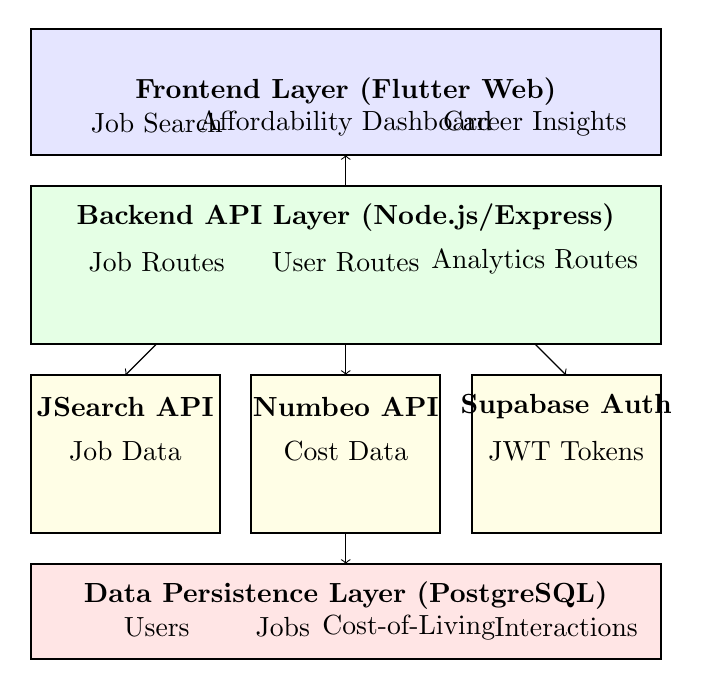
\begin{tikzpicture}[scale=0.8]
    \draw[thick, fill=blue!10] (0,8) rectangle (10,10);
    \node at (5,9) {\textbf{Frontend Layer (Flutter Web)}};
    \node at (2,8.5) {Job Search};
    \node at (5,8.5) {Affordability Dashboard};
    \node at (8,8.5) {Career Insights};
    
    \draw[thick, fill=green!10] (0,5) rectangle (10,7.5);
    \node at (5,7) {\textbf{Backend API Layer (Node.js/Express)}};
    \node at (2,6.3) {Job Routes};
    \node at (5,6.3) {User Routes};
    \node at (8,6.3) {Analytics Routes};
    
    \draw[thick, fill=yellow!10] (0,2) rectangle (3,4.5);
    \node at (1.5,4) {\textbf{JSearch API}};
    \node at (1.5,3.3) {Job Data};
    
    \draw[thick, fill=yellow!10] (3.5,2) rectangle (6.5,4.5);
    \node at (5,4) {\textbf{Numbeo API}};
    \node at (5,3.3) {Cost Data};
    
    \draw[thick, fill=yellow!10] (7,2) rectangle (10,4.5);
    \node at (8.5,4) {\textbf{Supabase Auth}};
    \node at (8.5,3.3) {JWT Tokens};
    
    \draw[thick, fill=red!10] (0,0) rectangle (10,1.5);
    \node at (5,1) {\textbf{Data Persistence Layer (PostgreSQL)}};
    \node at (2,0.5) {Users};
    \node at (4,0.5) {Jobs};
    \node at (6,0.5) {Cost-of-Living};
    \node at (8.5,0.5) {Interactions};
    
    \draw[->] (5,7.5) -- (5,8);
    \draw[->] (2,5) -- (1.5,4.5);
    \draw[->] (5,5) -- (5,4.5);
    \draw[->] (8,5) -- (8.5,4.5);
    \draw[->] (5,2) -- (5,1.5);
\end{tikzpicture}
\caption{High-Level System Architecture Overview}
\label{fig:architecture}
\end{figure}

\section{System Components}

\subsection{Job Discovery Module}

The Job Discovery Module aggregates real-time job listings from multiple sources, normalizes heterogeneous data formats, and exposes a unified job catalog through RESTful endpoints.

\textbf{Responsibilities:}
\begin{itemize}
    \item Fetch live job listings from the JSearch API based on user search queries, location filters, and company preferences.
    \item Transform raw API responses into a standardized internal job schema, ensuring consistent field mapping across sources.
    \item Implement pagination and caching strategies to optimize API usage and reduce latency.
    \item Provide filtering and sorting capabilities on job attributes (role, company, salary range, tech stack, posting date).
\end{itemize}

\subsection{Affordability Analysis Module}

The Affordability Analysis Module integrates real-time cost-of-living data with salary information to produce personalized affordability scores.

\textbf{Responsibilities:}
\begin{itemize}
    \item Scrape current cost-of-living data from Numbeo for supported Indian cities, extracting rent, grocery, transportation, and utility costs.
    \item Implement an in-memory cache with configurable TTL (Time-To-Live) to minimize redundant API calls while maintaining data freshness.
    \item Calculate city-specific expense profiles based on user lifestyle preferences (single vs. family, urban vs. suburban).
    \item Compute affordability scores using a proprietary formula that correlates salary with cost of living.
\end{itemize}

\textbf{Affordability Score Formula:}

Let:
\begin{align*}
S &= \text{Annual salary (in INR)} \\
C &= \text{Annual cost of living (in INR)} \\
D &= \text{Disposable income} = S - C \\
T &= \text{Target disposable income threshold (user-defined, default ₹10 lakhs/year)}
\end{align*}

\begin{equation}
\text{Affordability Score} = \min\left(100, \frac{D}{T} \times 100\right)
\end{equation}

This formula yields a score from 0-100, where 100 represents excellent affordability and 0 represents poor affordability.

\subsection{Career Insights Module}

The Career Insights Module correlates job offers with user preferences, salary trends, and company reputation to generate personalized recommendations and career trajectory projections.

\subsection{User Management and Authentication Module}

The User Management Module handles user registration, authentication, profile management, and personalization preferences.

\section{AI Integration and Data Flow}

\subsection{Automated Data Alignment}

The system automatically aligns heterogeneous job data from multiple sources (JSearch API, internal database) into a unified schema.

\subsection{Affordability-Driven Ranking}

Rather than ranking jobs by recency or popularity, Salariann ranks results by affordability score, ensuring that the most financially viable opportunities appear first.

\subsection{Iterative Recommendation Refinement}

The system implements a feedback loop where user interactions are collected and used to refine recommendation models.

\section{Detailed Workflow of the System}

The following numbered steps trace a complete user journey from initial login through job discovery:

\begin{enumerate}
    \item \textbf{User Authentication}: The user navigates to the Salariann home page and signs in using email and password.
    
    \item \textbf{Profile Setup}: On first login, the user completes a profile questionnaire specifying lifestyle preferences.
    
    \item \textbf{Job Search Initiation}: The user enters a search query and selects one or more cities.
    
    \item \textbf{Real-Time Job Aggregation}: The backend receives the request and calls the JSearch API.
    
    \item \textbf{Data Transformation}: The backend transforms raw JSearch responses into the internal job schema.
    
    \item \textbf{Cost-of-Living Lookup}: For each job's city, the backend checks the in-memory cache for current cost-of-living data.
    
    \item \textbf{Affordability Scoring}: The backend computes an affordability score for each job.
    
    \item \textbf{Response Formatting}: The backend returns a JSON response containing the sorted job list.
    
    \item \textbf{Job Selection and Details}: The user clicks on a job card to view full details.
    
    \item \textbf{Application or Save}: The user either applies for the job or saves the job for later review.
\end{enumerate}

% ============================================================================
% CHAPTER 4: SYSTEM DESIGN
% ============================================================================
\chapter{System Design}

\section{System Architecture Diagram}

\begin{figure}[H]
\centering
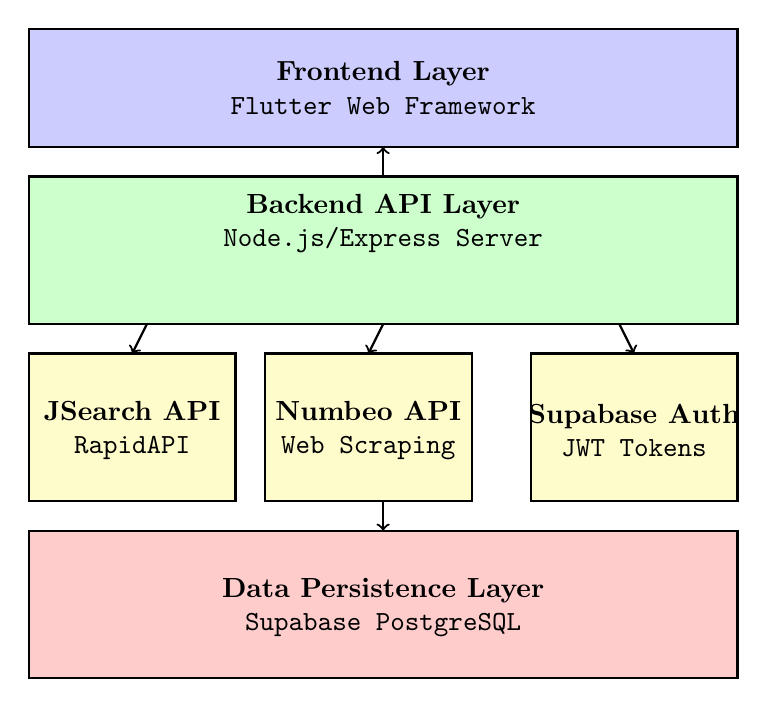
\begin{tikzpicture}[scale=0.75]
    \draw[thick, fill=blue!20] (0,10) rectangle (12,12);
    \node[align=center] at (6,11) {\textbf{Frontend Layer}\\\texttt{Flutter Web Framework}};
    
    \draw[thick, fill=green!20] (0,7) rectangle (12,9.5);
    \node[align=center] at (6,8.7) {\textbf{Backend API Layer}\\\texttt{Node.js/Express Server}};
    
    \draw[thick, fill=yellow!20] (0,4) rectangle (3.5,6.5);
    \node[align=center] at (1.75,5.2) {\textbf{JSearch API}\\\texttt{RapidAPI}};
    
    \draw[thick, fill=yellow!20] (4,4) rectangle (7.5,6.5);
    \node[align=center] at (5.75,5.2) {\textbf{Numbeo API}\\\texttt{Web Scraping}};
    
    \draw[thick, fill=yellow!20] (8.5,4) rectangle (12,6.5);
    \node[align=center] at (10.25,5.2) {\textbf{Supabase Auth}\\\texttt{JWT Tokens}};
    
    \draw[thick, fill=red!20] (0,1) rectangle (12,3.5);
    \node[align=center] at (6,2.2) {\textbf{Data Persistence Layer}\\\texttt{Supabase PostgreSQL}};
    
    \draw[->, thick] (6,9.5) -- (6,10);
    \draw[->, thick] (2,7) -- (1.75,6.5);
    \draw[->, thick] (6,7) -- (5.75,6.5);
    \draw[->, thick] (10,7) -- (10.25,6.5);
    \draw[->, thick] (6,4) -- (6,3.5);
\end{tikzpicture}
\caption{Detailed System Architecture Diagram}
\label{fig:detailed_arch}
\end{figure}

\section{Data Flow Diagram}

\subsection{Level 0 Context Diagram}

\begin{figure}[H]
\centering
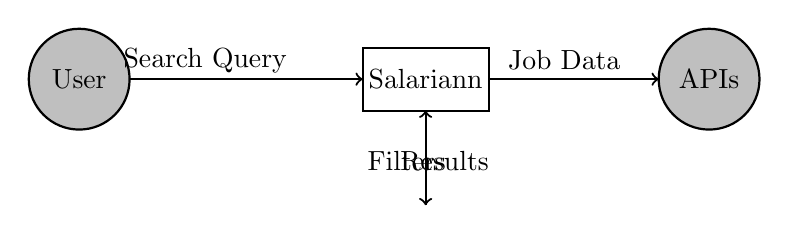
\begin{tikzpicture}[scale=0.8]
    \draw[circle, thick, fill=lightgray] (1,5) circle (0.8);
    \node at (1,5) {User};
    
    \draw[circle, thick, fill=lightgray] (11,5) circle (0.8);
    \node at (11,5) {APIs};
    
    \draw[thick, fill=white] (5.5,4.5) rectangle (7.5,5.5);
    \node at (6.5,5) {Salariann};
    
    \draw[->, thick] (1.8,5) -- (5.5,5);
    \node at (3,5.3) {Search Query};
    
    \draw[->, thick] (7.5,5) -- (10.2,5);
    \node at (8.7,5.3) {Job Data};
    
    \draw[->, thick] (6.5,4.5) -- (6.5,3);
    \node at (6.8,3.7) {Results};
    
    \draw[->, thick] (6.5,3) -- (6.5,4.5);
    \node at (6.2,3.7) {Filters};
\end{tikzpicture}
\caption{Context Diagram (Level 0 DFD)}
\label{fig:dfd_l0}
\end{figure}

\subsection{Level 1 Detailed Data Flow Diagram}

\begin{figure}[H]
\centering
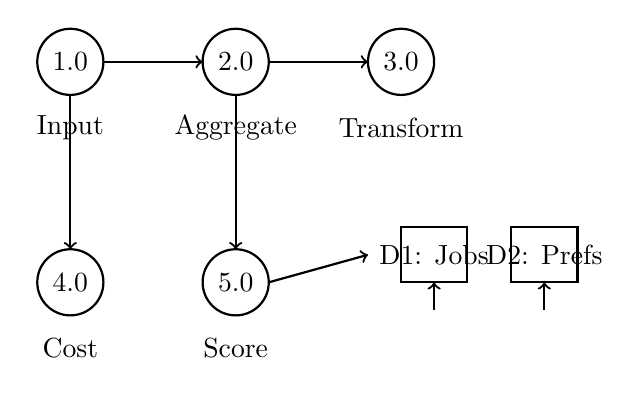
\begin{tikzpicture}[scale=0.7]
    \draw[circle, thick] (2,8) circle (0.6);
    \node at (2,8) {1.0};
    \node at (2,6.8) {Input};
    
    \draw[circle, thick] (5,8) circle (0.6);
    \node at (5,8) {2.0};
    \node at (5,6.8) {Aggregate};
    
    \draw[circle, thick] (8,8) circle (0.6);
    \node at (8,8) {3.0};
    \node at (8,6.8) {Transform};
    
    \draw[circle, thick] (2,4) circle (0.6);
    \node at (2,4) {4.0};
    \node at (2,2.8) {Cost};
    
    \draw[circle, thick] (5,4) circle (0.6);
    \node at (5,4) {5.0};
    \node at (5,2.8) {Score};
    
    \draw[rectangle, thick] (8,4) rectangle (9.2,5);
    \node at (8.6,4.5) {D1: Jobs};
    
    \draw[rectangle, thick] (10,4) rectangle (11.2,5);
    \node at (10.6,4.5) {D2: Prefs};
    
    \draw[->, thick] (2.6,8) -- (4.4,8);
    \draw[->, thick] (5.6,8) -- (7.4,8);
    \draw[->, thick] (2,7.4) -- (2,4.6);
    \draw[->, thick] (5,7.4) -- (5,4.6);
    \draw[->, thick] (5.6,4) -- (7.4,4.5);
    \draw[->, thick] (8.6,3.5) -- (8.6,4);
    \draw[->, thick] (10.6,3.5) -- (10.6,4);
\end{tikzpicture}
\caption{Detailed Data Flow Diagram (Level 1 DFD)}
\label{fig:dfd_l1}
\end{figure}

\section{UML Diagrams}

\subsection{Use Case Diagram}

\begin{figure}[H]
\centering
\begin{tikzpicture}[scale=0.8]
    \draw[thick, rectangle] (2,1) rectangle (8,7);
    \node at (5,6.7) {Salariann System};
    
    \draw[ellipse, thick] (3.5,5.5) ellipse (1,0.5);
    \node at (3.5,5.5) {Search Jobs};
    
    \draw[ellipse, thick] (5,5.5) ellipse (1,0.5);
    \node at (5,5.5) {View Details};
    
    \draw[ellipse, thick] (6.5,5.5) ellipse (1,0.5);
    \node at (6.5,5.5) {Save Job};
    
    \draw[ellipse, thick] (4,3.5) ellipse (1,0.5);
    \node at (4,3.5) {Calculate};
    
    \draw[ellipse, thick] (6,3.5) ellipse (1,0.5);
    \node at (6,3.5) {View Insights};
    
    \draw[circle, thick, fill=lightgray] (0.5,4) circle (0.5);
    \node at (0.5,4) {User};
    
    \draw[circle, thick, fill=lightgray] (9,4) circle (0.5);
    \node at (9,4) {APIs};
    
    \draw[-] (1,4) -- (2,5.5);
    \draw[-] (1,4) -- (2,3.5);
    \draw[-] (8,4) -- (8,5.5);
\end{tikzpicture}
\caption{Use Case Diagram}
\label{fig:usecase}
\end{figure}

\subsection{Class Diagram}

\begin{table}[H]
\centering
\caption{Key Classes and Their Responsibilities}
\label{tab:classes}
\begin{tabular}{|l|l|l|}
\hline
\textbf{Class} & \textbf{Key Attributes} & \textbf{Key Methods} \\
\hline
User & id, email, displayName, lifestyle & signUp(), login(), updateProfile() \\
\hline
Job & id, title, company, salary, city & getDetails(), calculateScore() \\
\hline
Company & id, name, logoUrl, website & getProfile(), getReviews() \\
\hline
CostOfLiving & id, city, rent, grocery, transport & getProfile(), updateData() \\
\hline
AffordabilityScore & jobId, userId, score & calculate(), getBreakdown() \\
\hline
\end{tabular}
\end{table}

\section{Database Schema}

\begin{table}[H]
\centering
\caption{Database Schema and Storage Strategy}
\label{tab:schema}
\begin{tabular}{|l|l|p{6cm}|}
\hline
\textbf{Table} & \textbf{Type} & \textbf{Description} \\
\hline
users & PostgreSQL & User profiles with authentication data \\
\hline
jobs & PostgreSQL & Job listings from JSearch and local sources \\
\hline
companies & PostgreSQL & Company information and metadata \\
\hline
cost\_of\_living & PostgreSQL & City-specific cost-of-living data \\
\hline
user\_job\_interactions & PostgreSQL & User behavior tracking and analytics \\
\hline
reviews & PostgreSQL & User-submitted company reviews \\
\hline
\end{tabular}
\end{table}

\section{Entity Relationship Diagram}

\begin{figure}[H]
\centering
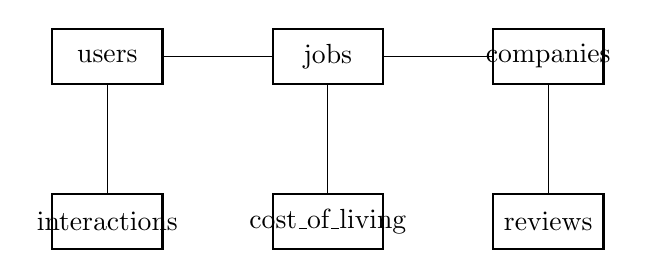
\begin{tikzpicture}[scale=0.7]
    \draw[rectangle, thick] (1,8) rectangle (3,9);
    \node at (2,8.5) {users};
    
    \draw[rectangle, thick] (5,8) rectangle (7,9);
    \node at (6,8.5) {jobs};
    
    \draw[rectangle, thick] (9,8) rectangle (11,9);
    \node at (10,8.5) {companies};
    
    \draw[rectangle, thick] (5,5) rectangle (7,6);
    \node at (6,5.5) {cost\_of\_living};
    
    \draw[rectangle, thick] (1,5) rectangle (3,6);
    \node at (2,5.5) {interactions};
    
    \draw[rectangle, thick] (9,5) rectangle (11,6);
    \node at (10,5.5) {reviews};
    
    \draw[-] (3,8.5) -- (5,8.5);
    \draw[-] (7,8.5) -- (9,8.5);
    \draw[-] (6,8) -- (6,6);
    \draw[-] (2,8) -- (2,6);
    \draw[-] (10,8) -- (10,6);
    \draw[-] (6,5) -- (6,5);
\end{tikzpicture}
\caption{Entity Relationship Diagram}
\label{fig:erd}
\end{figure}


% ============================================================================
% IMPORT CHAPTERS FROM PART 3 (Chapters 5-8 + Appendices)
% ============================================================================
\input{SALARIANN_REPORT_PART3_CHAPTERS.tex}

\end{document}
